% Created 2025-04-29 Tue 19:46
% Intended LaTeX compiler: pdflatex
\documentclass[11pt]{article}
\usepackage[utf8]{inputenc}
\usepackage[T1]{fontenc}
\usepackage{graphicx}
\usepackage{longtable}
\usepackage{wrapfig}
\usepackage{rotating}
\usepackage[normalem]{ulem}
\usepackage{amsmath}
\usepackage{amssymb}
\usepackage{capt-of}
\usepackage{hyperref}
\usepackage{minted}
\usepackage{tikz}
\usetikzlibrary{angles, quotes}
\author{Hankertrix}
\date{\today}
\title{Math Module 4A Notes}
\hypersetup{
 pdfauthor={Hankertrix},
 pdftitle={Math Module 4A Notes},
 pdfkeywords={},
 pdfsubject={},
 pdfcreator={Emacs 30.1 (Org mode 9.7.11)}, 
 pdflang={English}}
\begin{document}

\maketitle
\setcounter{tocdepth}{2}
\tableofcontents \clearpage\section{Definitions}
\label{sec:org28eab79}

\subsection{Indefinite integral}
\label{sec:orge740ebf}
An indefinite integral represents the collection of \textbf{all} antiderivatives of a function \(f(x)\).
\[\int f(x) \, dx\]
\subsubsection{Example}
\label{sec:org644b2dc}
We know that all the antiderivatives of the function \(f(x) = 2x\) have the form \(F(x) = x^2 + C\), where \(C\) is an arbitrary constant, so we express this fact by writing:
\[\int 2x \, dx = x^2 + C\]
\subsection{Trigonometric polynomial}
\label{sec:orgad53544}
A trigonometric polynomial is a sum of terms like:
\[\cos^m x \sin^n x\]
\subsection{Division algorithm}
\label{sec:org5b7d95a}
Let \(a, b \in \mathbb{Z}, b \ne 0\). Then there exist unique \(q, r \in \mathbb{Z}\) such that:
\[a = qb + r, \quad 0 \le r \le |b|\]

The integer \(q\) above is called the \textbf{quotient} and \(r\) is called the \textbf{remainder}, when \(a\) is divided by \(b\).
\subsection{Polynomial division}
\label{sec:org9a7fc67}
Dividing a \textbf{polynomial} \(P(x)\) by a \textbf{polynomial} \(Q(x)\) means finding polynomials \(q(x), r(x)\) such that:
\[P(x) = q(x) Q(x) + r(x), \quad \text{deg } r(x) < \text{deg } Q(x)\]

\(q\) is called the \textbf{quotient} and \(r\) is the \textbf{remainder} when \(p\) is divided by \(Q\).
\section{List of basic indefinite integrals}
\label{sec:orga1a80a7}
\[\text{1. } \int x^a \, dx = \frac{x^{a + 1}}{a + 1} + C \text{ for } a \ne -1\]
\begin{align*}
\text{2. } \int \frac{1}{x} \, dx &= \ln |x| + C \\
&= \ln x + C \text{ for } x > 0 \\
&= \ln (-x) + C \text{ for } x < 0
\end{align*}
\[\text{3. } \int e^x \, dx = e^x + C\]
\[\text{4. } \int \sin x \, dx = - \cos x + C\]
\[\text{5. } \int \cos x \, dx = \sin x + C\]
\[\text{6. } \int \frac{1}{\cos^2 x} \, dx = \tan x + C\]
\[\text{7. } \int \frac{1}{\sin^2 x} \, dx = - \cot x + C\]
\[\text{8. } \int \frac{1}{1 + x^2} \, dx = \arctan x + C\]
\[\text{9. } \int \frac{1}{\sqrt{1 - x^2}} \, dx = \arcsin x + C\]
\section{Integration by parts}
\label{sec:orge736479}
Since:
\[\frac{d}{dx} f(x) g(x) = f'(x) g(x) + f(x) g'(x)\]

We get:
\[f(x) g(x) + C = \int f'(x) g(x) \, dx + \int f(x) g'(x) \, dx\]

I.e.
\[\int f(x) g'(x) \, dx = f(x) g(x) - \int f'(x) g(x) \, dx\]
\section{Change of variables (substitution)}
\label{sec:org4bd54a1}
By the chain rule we have:
\[\frac{d}{dx} f(g(x)) = f'(g(x)) g'(x)\]

So:
\[\int f'(g(x)) g'(x) \, dx = f(g(x)) + C\]

Using the notation:
\[u = g(x), \ du = g'(x) \, dx\]

We get:
\[\int f'(u) \, du = f(u) + C\]

The trick below works well if we can identify \(g'(x)\) as a factor of the integrand.
\[\int f'(g(x)) g'(x) \, dx = \left[ \begin{gathered} u = g(x) \\ du = g'(x) \, dx \end{gathered} \right] = \int f'(u) \, du\]
\section{Inverse substitution}
\label{sec:orgbf38df0}
Sometimes, an inverse substitution \(x = h(t), \, dx = h'(t) \, dt\), works well. In inverse substitutions, we want \(h\) to be one-to-one so that \(t = h^{-1} (x)\).

\[\int f(x) \, dx = \int f(h(t)) h'(t) \, dt\]
\subsection{Substitution for \(\sqrt{1 - x^2}\)}
\label{sec:orgac7ee1a}
Find \(\int \sqrt{1 - x^2} \, dx\). For integrals where \(\sqrt{1 - x^2}\) appears and there is no other obvious way forward, the follow idea often works:

\begin{center}
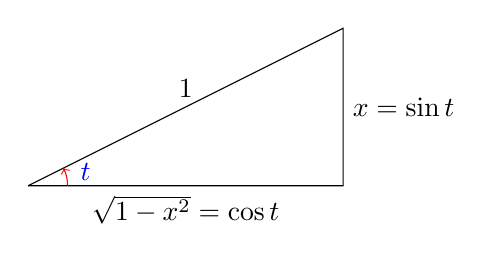
\begin{tikzpicture}

% The coordinates of the points of the triangle
\coordinate (a) at (0,0);
\coordinate (b) at (4,0);
\coordinate (c) at (4,2);

% The triangle
\draw (a) -- (b) node[midway, below]{$\sqrt{1 - x^2} = \cos t$} -- (c) node[midway, right]{$x = \sin t$} -- (a) node[midway, left, above]{1};

% The angle
\pic [draw=red, text=blue, ->, "$t$", angle eccentricity=1.5] {angle = b--a--c};
\end{tikzpicture}
\end{center}

The inverse substitution:
\[x = \sin t\]
\[\sqrt{1 - x^2} = \cos t\]

In general:
\[\cos t = \pm \sqrt{1 - \sin^2 t} = \pm \sqrt{1 - x^2}\]

But for our inverse substitution, we have:
\[t = \arcsin x \in \left[- \frac{\pi}{2}, \frac{\pi}{2} \right]\]

So:
\[\cos t \ge 0\]
\[\cos t = \sqrt{1 - x^2}\]

The equations we have:
\[x = \sin t\]
\[dx = \cos t \, dt\]
\[\sqrt{1 - x^2} = \cos t\]

Finding \(\int \sqrt{1 - x^2} \, dx\):
\begin{align*}
\int \sqrt{1 - x^2} \, dx &= \int cos^2 t \, dt \\
&= \int \frac{1 + \cos 2t}{2} \, dt \\
&= \frac{t}{2} + \frac{\sin 2t}{4} + C \\
&= \frac{t}{2} + \frac{2 \sin t \cos t}{4} + C \\
&= \frac{1}{2} \arcsin x + \frac{2 \cdot 2x \sqrt{1 - x^2}}{4} + C \\
&= \frac{1}{2} \arcsin x + \frac{1}{2}x \sqrt{1 - x^2} + C \\
\end{align*}

\newpage
\subsection{Substitution for \(\sqrt{x^2 + 1}\)}
\label{sec:org4510a58}

\begin{center}
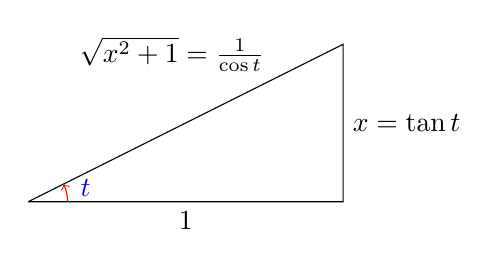
\begin{tikzpicture}

% The coordinates of the points of the triangle
\coordinate (a) at (0,0);
\coordinate (b) at (4,0);
\coordinate (c) at (4,2);

% The triangle
\draw (a) -- (b) node[midway, below]{1} -- (c) node[midway, right]{$x = \tan t$} -- (a) node[midway, left, above, yshift = 1.5em, xshift = -0.5em]{$\sqrt{x^2 + 1} = \frac{1}{\cos t}$};

% The angle
\pic [draw=red, text=blue, ->, "$t$", angle eccentricity=1.5] {angle = b--a--c};
\end{tikzpicture}
\end{center}

In general,
\begin{align*}
\frac{1}{\cos^2 t} &= \frac{\sin^2 t + \cos^2 t}{\cos ^2 t} \\
&= \tan^2 t + 1 \\
&= x^2 + 1
\end{align*}

So:
\[\frac{1}{\cos t} = \pm \sqrt{x^2 + 1}\]

But for our inverse substitution, we take:
\[t = \arctan x \in \left(- \frac{\pi}{2}, \frac{\pi}{2} \right)\]

So \(\cos t > 0\), i.e.
\[\frac{1}{\cos t} = \sqrt{x^2 + 1}\]

\newpage
\subsection{Substitution for \(\sqrt{x^2 - 1}\)}
\label{sec:org9ea3340}

\begin{center}
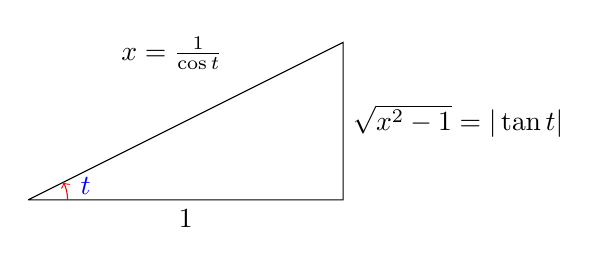
\begin{tikzpicture}

% The coordinates of the points of the triangle
\coordinate (a) at (0,0);
\coordinate (b) at (4,0);
\coordinate (c) at (4,2);

% The triangle
\draw (a) -- (b) node[midway, below]{1} -- (c) node[midway, right]{$\sqrt{x^2 - 1} = |\tan t|$} -- (a) node[midway, left, above, yshift = 1.5em, xshift = -0.5em]{$x = \frac{1}{\cos t}$};

% The angle
\pic [draw=red, text=blue, ->, "$t$", angle eccentricity=1.5] {angle = b--a--c};
\end{tikzpicture}
\end{center}

\begin{align*}
\sqrt{x^2 - 1} &= \sqrt{\frac{1}{\cos^2 t} - 1} \\
&= \sqrt{\frac{1 - \cos^2 t}{\cos^2 t}} \\
&= \sqrt{\frac{\sin^2 t}{\cos ^2 t}} \\
&= \sqrt{\tan^2 t} \\
&= |\tan t| = \begin{cases}
\tan t & \text{for } t \in \left[0, \frac{\pi}{2} \right) \\
- \tan t & \text{for } t \in \left(\frac{\pi}{2}, \pi \right]
\end{cases}
\end{align*}

\newpage
\section{Integration of trigonometric polynomials}
\label{sec:org616feb3}
These equations below are useful:
\[\cos^2 x = \frac{1 + \cos 2x}{2}\]
\[\sin^2 x = \frac{1 - \cos 2x}{2}\]
\subsection{Even powers}
\label{sec:orga0c87fe}
If all powers are even, we can use those formulas to reduce its degree.

\begin{align*}
\int \cos^2 x \sin^2 x \, dx &= \int \frac{1 + \cos 2x}{2} \cdot \frac{1 - \cos 2x}{2} \, dx \\
&= \frac{1}{4} \int (1 - \cos^2 2x) \, dx \\
&= \frac{1}{4} \int \sin^2 2x \\
&= \frac{1}{8} \int (1 - \cos 4x) \, dx \\
&= \frac{1}{8} \left( x - \frac{\sin 4x}{4} \right) + C
\end{align*}

\newpage
\subsection{One odd power}
\label{sec:org7e20157}
If at least one power is odd, we can make a clever substitution.

\begin{align*}
\int \sin^3 x \cos^4 x \, dx &= \int \sin^2 x \cos^4 x \sin x \, dx \\
&= \int (1 - \cos^2 x) \cos^4 \sin x \, dx \\
&\quad \left[ \begin{gathered} u = \cos x \\ du = - \sin x \, dx \end{gathered} \right] \\
&= - \int (1 - u^2) u^4 \, du \\
&= - \int u^4 - u^6 \, du \\
&= \frac{u^7}{7} - \frac{u^5}{5} + C \\
&= \frac{\cos^7 x}{7} - \frac{\cos^5}{5} + C
\end{align*}
\section{Factoring polynomials}
\label{sec:org34c4e72}
Each polynomial \(Q(x)\) can be factorised:
\[Q(x) = A(x - x_1)(x - x_2) \cdots (x - x_n)\]

Where \(x_1, \ldots, x_n\) are the roots. Some \(x_i\) might be complex. But if the coefficients of \(Q\) are real, complex roots occur only in couples:
\[a - bi, \quad a + bi\]

For such pairs of complex roots, multiplying the corresponding factors gives:
\[(x - a + bi)(x - a - bi) = (x - a)^2 + b^2\]

So, any polynomial is a product of linear and quadratic polynomials, where each quadratic factor has no real root. The power of each factor in the product is called the \textbf{multiplicity}.
\section{Guessing roots}
\label{sec:org3ebd62e}
If a polynomial with integer coefficients has an integer root, we can guess it.


If all the coefficients of a polynomial \(Q(x)\) are integers and the root \(x\) is integer, then \(x\) divides the constant term.
\subsection{Example}
\label{sec:org7ebfb76}
Factorise \(Q(x) = x^5 - 2x^3 - 2x^2 - 3x - 2\).


Any integer root of \(Q\) must divide by \(-2\), so possible integer roots are \(\pm 1, \pm 2\). Substituting, we see that \(-1\) is a root, so \(x + 1\) is a factor of \(Q\).


Doing long division:
\[Q(x) = (x + 1)(x^4 - x^3 - x^2 - x - 2)\]

Again, any integer roots of \(x^4 - x^3 - x^2 - x - 2\) must divide by \(-2\) so again, possible integer roots are \(\pm 1, \pm 2\). Testing, we find that \(-1\) is a root, so we divide by \((x + 1)\) again.


Doing long division:
\begin{align*}
Q(x) &= (x + 1)(x^3 - x^2 - x - 2) \\
&= (x + 1)^2 (x^3 - 2x^2 + x - 2)
\end{align*}

Again, any integer roots of \(x^3 - 2x^2 + x - 2\) must divide by \(-2\) so again, possible integer roots are \(\pm 1, \pm 2\). Testing, we find that \(2\) is a root, so we divide by \((x - 2)\).


Doing long division:
\begin{align*}
Q(x) &= (x + 1)(x^3 - x^2 - x - 2) \\
&= (x + 1)^2 (x^3 - 2x^2 + x - 2) \\
&= (x + 1)^2 (x - 2) (x^2 + 1)
\end{align*}

Since \(x^2 + 1\) has no real roots, we are done.
\section{Integrating a rational function}
\label{sec:orgab12845}
Given a rational function:
\[f(x) = \frac{P(x)}{Q(x)} = \frac{x^n + a_{n - 1} x^{n - 1} + \cdots + a_0}{x^m + b_{m - 1} + \cdots + b_0}\]

A partial fraction is an expression from the following list:
\[\text{1. } Dx^k\]
\[\text{2. } \frac{C}{(x - c)^k}\]
\[\text{3. } \frac{Ax + B}{(x^2 + px + q)^k}, \text{ where the function } x^2 + px + q \text{ has no real root}\]
\subsection{Step 1}
\label{sec:orga25056b}
If deg \(P \ge \text{deg } Q\), divide \(P(x)\) by \(Q(x)\):
\begin{align*}
f(x) &= \frac{P(x)}{Q(x)} \\
&= \frac{q(x)Q(x) + r(x)}{Q(x)} \\
&= q(x) + \frac{r(x)}{Q(x)}
\end{align*}

\(q(x)\) is a polynomial, so it can be integrated.
\[\text{deg } r < \text{deg } Q\]
\subsection{Step 2}
\label{sec:org5d923a8}
Factorise \(Q(x)\) into linear and irreducible quadratic factors:
\[Q(x) = A(x - c_1)^{l_1} \cdots (x - c_\alpha)^{l_\alpha}[(x - a_1)^2 + b_1^2]^{q_1} \cdots [(x - a_\beta)^2 + b_\beta^2]^{q_\beta}\]
\subsection{Step 3}
\label{sec:org31d9836}
Each factor \((x - c)^l\) in \(Q(x)\), gives us partial fractions:
\[\frac{C_1}{x - c}, \frac{C_2}{(x - c)^2}, \cdots, \frac{C_l}{(x - c)^l}\]

And each factor \([(x - a)^2 + b^2]^q\) gives us partial fractions:
\[\frac{A_1 x + B_1}{(x - a)^2 + b^2}, \frac{A_2 x + B_2}{[(x - a)^2 +b^2]^2}, \cdots, \frac{A_q x + B_q}{[(x - a)^2 + b^2]^q}\]
\subsection{Example}
\label{sec:org3283176}
Find:
\[\int \frac{x^6 + 2x^4 + x^2 + x + 1}{x^ 5 + 2x^3 + x} \, dx\]

First step:
\[\frac{x(x^5 + 2x^3 + x) + x + 1}{x^5 + 2x^3 + x} = x + \frac{x + 1}{x^5 + 2x^3 + x}\]

Second step:
\begin{align*}
x^5 + 2x^3 + x &= x(x^4 + 2x^2 + 1) \\
&= x(x^2 + 1)^2
\end{align*}

Third step:
\[\frac{x + 1}{x(x^2 + 1)^2} = \frac{a}{x} + \frac{bx + c}{x^2 + 1} + \frac{dx + e}{(x^2 + 1)^2}\]

Calculating, we have:
\begin{align*}
&\frac{a}{x} + \frac{bx + c}{x^2 + 1} + \frac{dx + e}{(x^2 + 1)^2} \\
&= \frac{a(x^4 + 2x^2 + 1) + x(bx + c)(x^2 + 1) + x(dx + e)}{x(x^2 + 1)^2} \\
&= \frac{(a + b)x^4 + cx^3 + (2a + b + d)x^2 + (c + e)x + a}{x(x^2 + 1)^2}
\end{align*}

Comparing coefficients with the original expression:
\[\frac{x + 1}{x(x^2 + 1)^2}\]

\begin{center}
\begin{tabular}{c c c c c c c c c c}
a  & + & b &   &   &   &   &   &   &= 0 \\
   &   &   &   & c &   &   &   &   &= 0 \\
2a & + & b &   &   & + & d &   &   &= 0 \\
   &   &   &   & c &   &   & + & e &= 1 \\
   &   &   &   &   &   &   &   & a &= 1
\end{tabular}
\end{center}

I.e.
\[a = 1, \ b = -1, \ c = 0, \ d = -1, \ e = 1\]

So the integrand is:
\[x + \frac{1}{x} - \frac{x}{x^2 + 1} - \frac{x}{(x^2 + 1)^2} + \frac{1}{(x^2 + 1)^2}\]

\[\int x \, dx = \frac{x^2}{2} + C_1\]
\[\int \frac{1}{x} \, dx = \ln |x| + C_2\]

\begin{align*}
\int \frac{x}{x^2 + 1} \, dx &= \left[ \begin{gathered} u = x^2 + 1 \\ du = 2x \, dx \end{gathered} \right] \\
&= \frac{1}{2} \int \frac{1}{u} \, du \\
&= \frac{1}{2} \ln |u| + C_3 \\
&= \frac{1}{2} \ln (x^2 + 1) + C_3
\end{align*}

\begin{align*}
\int \frac{x}{(x^2 + 1)^2} \, dx &= \left[ \begin{gathered} u = x^2 + 1 \\ du = 2x \, dx \end{gathered} \right] \\
&= \frac{1}{2} \int \frac{1}{u^2} \, du \\
&= - \frac{1}{2u} + C_4 \\
&= - \frac{1}{2(x^2 + 1)} + C_4
\end{align*}

\begin{align*}
\int 1 \cdot \frac{1}{x^2 + 1} \, dx &= \frac{x}{x^2 + 1} - \int x \cdot \frac{-2x}{(x^2 + 1)^2} \, dx \\
&= \frac{x}{x^2 + 1} + 2 \int \frac{x^2 + 1 - 1}{(x^2 + 1)^2} \, dx \\
&= \frac{x}{x^2 + 1} + 2 \int \frac{1}{x^2 + 1} \, dx - 2 \int \frac{1}{(x^2 + 1)^2} \, dx
\end{align*}

So:
\begin{align*}
\int \frac{1}{(x^2 + 1)^2} &= \frac{1}{2} \frac{x}{x^2 + 1} + \frac{1}{2} \int \frac{1}{x^2 + 1} \, dx \\
&= \frac{1}{2} \frac{x}{x^2 + 1} + \frac{1}{2} \arctan x + C_5
\end{align*}

Wrapping it all up:
\begin{align*}
&\int \frac{x^6 + 2x^4 + x^2 + x + 1}{x^5 + 2x^3 + x} \, dx \\
&= \frac{x^2}{2} + \ln |x| - \frac{1}{2} \ln (1 + x^2) + \frac{1}{2(1 + x^2)} + \frac{x}{2(1 + x^2)} + \frac{1}{2} \arctan x + C
\end{align*}
\end{document}
